% latex sa1.tex
% dvisvgm --no-fonts --exact --bbox=papersize --output=sa1.svg sa1.dvi
\documentclass[tikz,border=0pt]{standalone}
\usepackage{courier}
\begin{document}
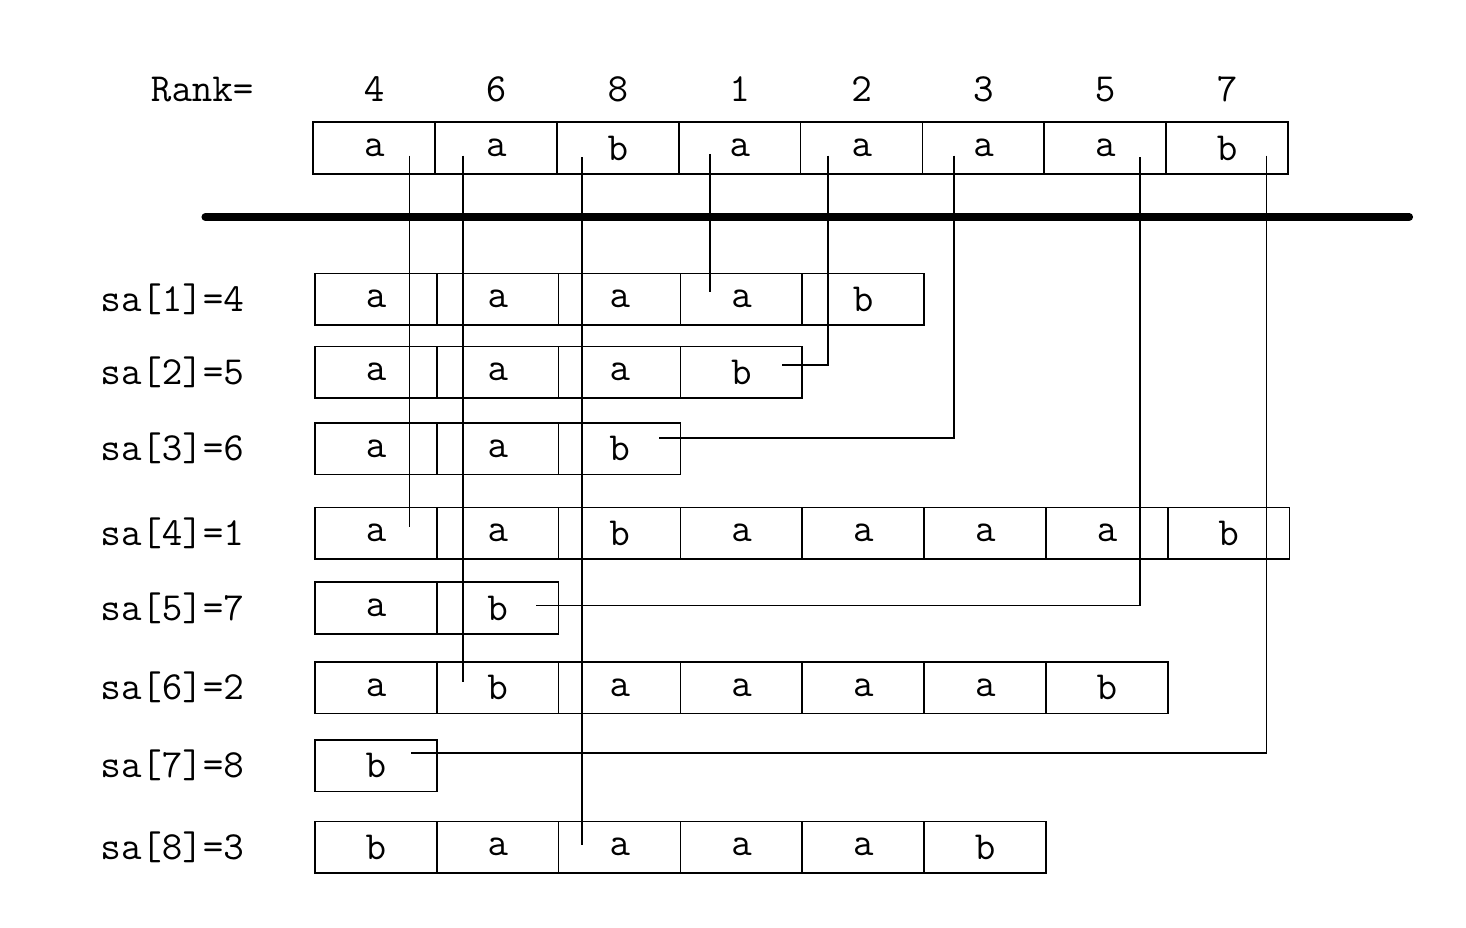
\begin{tikzpicture}[
    x=0.6pt,y=-0.6pt,
    font=\ttfamily\fontsize{14}{17}\selectfont,
    every node/.style={inner sep=0pt},
    line width=0.6pt
  ]
  % Coordinates retain the layout of the original 849 by 525 diagram.
  \path[use as bounding box] (0,0) rectangle (849,525);
  \node at (105,37) {Rank=};
  \foreach \rank[count=\i] in {4,6,8,1,2,3,5,7} {
    \node at ({172+(\i-0.5)*73.375},37) {\rank};
  }
  \foreach \letter[count=\i] in {a,a,b,a,a,a,a,b} {
    \draw ({172+(\i-1)*73.375},57) rectangle ({172+\i*73.375},88);
    \node at ({172+(\i-0.5)*73.375},72.5) {\letter};
  }
  \draw[line width=2.8pt,line cap=round] (107,114) -- (832,114);
  % The row labels and suffix boxes have the same positions and widths as
  % the original. The example string is aabaaaab.
  \foreach \rank/\start/\top/\suffix in {
      1/4/148/{a,a,a,a,b},
      2/5/192/{a,a,a,b},
      3/6/238/{a,a,b},
      4/1/289/{a,a,b,a,a,a,a,b},
      5/7/334/{a,b},
      6/2/382/{a,b,a,a,a,a,b},
      7/8/429/{b},
      8/3/478/{b,a,a,a,a,b}} {
    \node at (87,{\top+15.5}) {sa[\rank]=\start};
    \foreach \letter[count=\column] in \suffix {
      \draw ({173+(\column-1)*73.375},\top)
        rectangle ({173+\column*73.375},{\top+31});
      \node at ({173+(\column-0.5)*73.375},{\top+15.5}) {\letter};
    }
  }
  % Thin orthogonal guide lines map each original position to its sorted
  % suffix. They intentionally cross the boxes, as in the original image.
  \draw (230,77) -- (230,301);
  \draw (262,77) -- (262,394);
  \draw (334,78) -- (334,492);
  \draw (411,76) -- (411,159);
  \draw (482,77) -- (482,203) -- (454,203);
  \draw (558,77) -- (558,247) -- (380,247);
  \draw (670,78) -- (670,348) -- (306,348);
  \draw (746,77) -- (746,437) -- (231,437);
\end{tikzpicture}
\end{document}
